%%%%% Definitions of If- toggles
\newif\ifshowkexamples
\newif\ifshowoldstuff

%%%%% 
%\showkexamplestrue
%\showoldstufftrue

%%%%%
\documentclass{fithesis3}
\usepackage[T1]{fontenc}
\usepackage[utf8]{inputenc}
%\usepackage{syntax}
\usepackage{amsthm}
\usepackage{mathpartir}
\usepackage{listings}
\usepackage{subcaption}
\usepackage{xspace} % https://tex.stackexchange.com/a/17873
%\usepackage{todonotes}
%\usepackage{mathtime}

\usepackage[english]{babel}
\usepackage{float} % floating figures
\usepackage{minted}
%\usepackage{amsmath}
%\usepackage{amsfonts}
\usepackage{amssymb} % \rightsquigarrow etc
%\usepackage{makeidx}
%\usepackage{graphicx}

%\usepackage{k}
\usepackage[tight]{k}
% For unknown reason, the drawing is too 'white'
%\usepackage[style=math]{k}


\floatstyle{boxed} 
\restylefloat{figure}


%%%%%%%%%%%%%% Thesis metadata %%%%%%%%%%%%%%%
\thesissetup{
title = {An Executable Formal Semantics of C++},
TeXtitle = {An Executable Formal Semantics of C++},
author = {Jan Tušil},
keywords = {C++ semantics k-framework},
TeXkeywords = {C++ semantics k-framework},
advisor = {Jan Strejček},
gender = {m},
type = {mgr},
faculty = {fi},
%abstract = {Here will be an abstract},
%thanks = {Special thanks to...}
%bib = {references.bib}
}

%\addbibresource{references.bib}

%% Some math aliases
\newcommand{\var}[1]{\mathit{#1}\xspace}
\newcommand{\kast}{\texttt{kast}\xspace}
\newcommand{\krun}{\texttt{krun}\xspace}
\newcommand{\kompile}{\texttt{kompile}\xspace}
\newcommand{\kdoc}{\texttt{kdoc}\xspace}
\newcommand{\clangKast}{\texttt{clang-kast}\xspace}
\newcommand{\kcc}{\texttt{kcc}\xspace}
\newcommand{\Project}{Project\xspace}

% Notes about the 'k' package
% \ka{rule x => y} - inline K in ascii format
% \begin{asciik} rule x => y \end{asciik} - K ascii environment
% Displaying open/closed bubbles
% \kall{1}{2}{3}, \kprefix{1}{2}{3}, \ksuffix{1}{2}{3}, and \kmiddle{1}{2}{3}

\lstset {
	basicstyle=\footnotesize\ttfamily
}

\begin{document}

\chapter{Introduction}

Writing correct software is hard.
%Software verification is hard.
Although formal methods for software verification are being developed, there are few high quality tools on the market. One particular problem is that in order to create a~production-ready tool, it is not enough to understand formal methods; the developers also need to understand the precise semantics of the selected programming language.

% Knowledge of precise semantics of the selected programming language is needed.
In recent years, a~platform named ,,\K framework'' is gaining popuparity. The platform is based on the idea that formal, executable language semantics can be used to derive a~large variety of tools, including interpreters, debuggers, model checkers or deductive program verifiers~\cite{rosu-2017-marktoberdorf} (see Figure~\ref{kidea}). Tool developers, skilled in a~particular area of formal methods, can work inside their area of expertise and developing language independent tools, while leaving language details to someone else. Thus, a~separation of concerns is achieved.

% TODO sem obrazek

\begin{figure}[h]
\centering
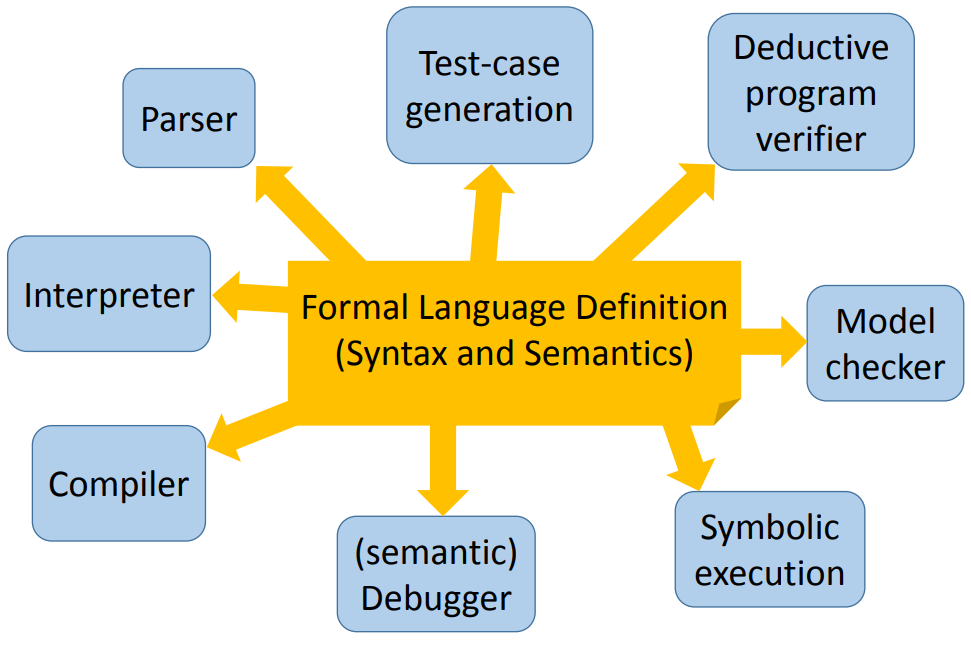
\includegraphics[width=0.7\linewidth]{img/kidea.png}
\caption{The idea behind \K. Adopted from~\cite{rosu-2015-meseguer}.}
\label{kidea}
% The image is simply print-screen-ed. Je to ok? A muzu rikat, ze jsem ho adoptoval?
\end{figure}

\K framework has been successfully used to give formal semantics to a~varienty of languages, including Java~\cite{bogdanas-rosu-2015-popl}, Python, Javascript~\cite{park-stefanescu-rosu-2015-pldi}, and C~\cite{ellison-2012-thesis,hathhorn-ellison-rosu-2015-pldi}, all of which is publicly available. The C semantics has been used to create RV-Match, a~,,tool for checking C programs for
undefined behavior and other common programmer mistakes''~\cite{guth-hathhorn-saxena-rosu-2016-cav}.  At the time of writing, the C semantics is being extended to support C++; the C++ support is also the focus of this thesis.

The thesis originally aimed to implement whichever language features needed to be done, as the C++ language is complex and the C++ semantics is still highly incomplete. As the work progressed, two features were selected to be implemented: \textit{enumerations} and \textit{constant expressions}. It went out that the two features play together rather nicely: C++ allows enumerators to be initialized with constant expressions, so enumerations can be used to test the implementation of constant expressions. 

Enumerations were chosen because of their relative simplicity: it is a~purely compile-time feature, which does not interfere much with other language features; it exists in the language from its beginning, and \textit{scoped enumerations} introduced in C++11 are even simpler both from language and user point of view (the legacy C-style enumerations still need to be supported, though).

\textit{Constant expressions}, on the contrary, had undergone a~deep change in C++11, which allowed a~restricted set of runtime computations to happen in the compilation time; the future revisions released the restrictions to the point that in C++17, almost arbitrary side effect free computations can happen in the time of compilation. One could reasonably expect that in order to implement constant expressions, a~more fundamental change to the semantics have to be done.
% (TODO tohle asi prijde dat do vice minuleho casu).
 
%"ukazalo se"
%(TODO zminit, ze za tim je ten 'constexpr' keyword).

The purpose of this text is to describe the implementation of the aforementioned features. The rest of the document is organized as follows:
\begin{enumerate}
\item introduction of the project of C/C++ semantics
\item description of the involved concepts
\item outline of the general architecture of the project
\item discussion of implementation of enums
\item discussion of implementation of constant expressions
\end{enumerate}

From this point on, we will write ,,\Project'' instead of ,,the C/C++ semantics in K''.

% at first, the project of C/C++ semantics is introduced; then the concepts involved are described in greater depth; then a~general architecture of the project of C/C++ semantics is outlined, followed by a~more detailed description of the parts related to the selected features. A discussion of details of the implementation...

%TODO pouzit figure 2 z PLDI'15, ACM. 2015.


% TODO dat jako prilohu k diplomce virtualku s nainstalovanym prostredim.
% TODO zminit prekazky pri vyvoji: pomala kompilace, nedeterminismus?

\chapter{Background}
This chapter intends to give a~brief overview of the \K framework, the C++ language, and the \Project.
The level of detail here is necessary to understand the description of the Implementation section and does not go much deeper; an inquisitive reader is encouraged to go through the K tutorial. % And read the Standard, and stack overflow, ...

\section{K framework}

%The purpose of this section is to give an overview of \K semantic framework. First subsection shows how \K can be used to describe language semantics in an operational manner; the second subsections contains an overview of various \K tools, including debugger, as well as a~brief introduction of \K abstract syntax; and the last subsection discuss in more detail various aspects of \K, including matching and reachability logic.
%
%\subsection{Idea}
%Mozna neni treba, mozna ze 
%\K framework idea - see their image.
%
%%We have to also mention that K framework can parse concrete syntax but it can also be used with an external parser.
%
%
%% KAst
%% 
%
%% Taky bych chtel popsat, jake nastroje K framework nabizi, z ceho se sklada apod. Ale ze aktualni prochazi rekonstrukci, takze nektere vlastnosti nefunguji. Pdf dokumentace ze semantiky. Obycejny interpreter, model checker, ...
%


\paragraph{K And Operational semantics}

%TODO reference some courses and lecture notes for small-step structural operational semantics
%TODO cite the k tutorial.

%TODO rozlisovat mezi 'language definition' - tim budu vzdycky oznacovat konkretni semantiku v K, a~proste semantikou.

In the \K framework, languages are described in a~style commonly known as \textit{operational semantics}. For any language $\var{L}$, when $\var{L}$ is given a~particular definition $\var{D}$ in \K framework, then $\var{D}$ assigns to every program in $\var{L}$ a~transition system $( \var{Cfg}, \rightarrow )$. Here $\var{Cfg}$ denotes a~set of program configurations and $\rightarrow$ is a~binary relation over $\var{Cfg}$; the relation is called a~,,transition relation'' and its elements are ,,transitions''. %Transitions correspond to computational steps; the existence of a~transition between two given configurations is determined by some kind of deductive system., or by pattern matching rewriting rules to the configurations (in case of \K).

%TODO an image of a~transition system

The configurations are not abstract, but they have an internal structure, which depends on the definition $\var{D}$. For a~simple imperative language, similar to the language IMP defined in the K tutorial~\cite{k-tutorial}, the configurations may consists of a~,,program'' part and a~,,data'' part.

\subsection{Terms}

The program part can be represented as a~term. \K allows to define a~multisorted algebraic signature $(S, \Sigma)$; closed terms over this signature forms a~(multisorted) term algebra. One may then choose a~particular sort $s \in \Sigma$ and declare the set of all programs to be the set of all closed terms of the sort $s$.

Sorts are defined using \texttt{syntax} keyword. The definition
\begin{lstlisting}
syntax H
syntax H ::= world()
syntax H ::= hello(H,H)
\end{lstlisting}
defines sort \texttt{H} and a~nullary constructor \texttt{world} and a~binary constructor \texttt{hello} of that sort. Uknown sorts on the left hand side of the operator~\texttt{::=} are automatically defined, and when defining multiple constructors for one sort, the right hand sides can be chained with the operator~\texttt{|}. The definition above is therefore equivalent to the following definition:
\begin{lstlisting}
syntax H ::= world() | hello(H,H)
\end{lstlisting}
Furthermore, \K allows the sort constructors to be given in an infix syntax and to contain ,,special'' symbols. Therefore, instead of
\begin{lstlisting}
syntax G ::= unit() | add(G, G) | inv(G)
\end{lstlisting}
it is possible to write
\begin{lstlisting}
syntax G ::= ".G" | G "+" G | "-" G
\end{lstlisting}
to describe the signature of groups. \K also supports subsorting; the following definition makes the sort \texttt{Int} a~subsort of the sort \texttt{Real}:
\begin{lstlisting}
syntax Real ::= Int
\end{lstlisting}

\begin{figure}[h]
\begin{lstlisting}
syntax AExp  ::= Int | Id
               | AExp "+" AExp
syntax BExp  ::= Bool
               | AExp "<=" AExp
               | "!" BExp
               | BExp "&&" BExp
               | "(" BExp ")"
syntax Block ::= "{" "}"
               | "{" Stmt "}"
syntax Stmt  ::= Block
               | Id "=" AExp ";"
               | "while" "(" BExp ")" Block
               | Stmt Stmt
syntax Pgm   ::= Stmt
\end{lstlisting}
\caption{A definition of an algebraic signature of the IMP.}
\label{impSyntax}
\end{figure}

\K is distributed together with a~basic library; together they provide a~number of pre-defined sorts, including \texttt{Id} \texttt{Int}, \texttt{Bool}, \texttt{List}, and \texttt{Map}. The \texttt{Id} is a~sort of C-style identifiers, the other names are rather self-explanatory. With use of these sorts, an algebraic signature of the IMP language can be defined as in Figure~\ref{impSyntax}. From the definition, \textit{arithmetic expressions} (represented by the sort \texttt{AExp}) are integers, identifiers, and sums of other arithmetic expressions; the arithmetic expressions can be compared to create \textit{boolean expressions} are boolean constants, and so on.

\subsection{Configurations}

A part of the program configuration can be stored in a~\textit{cell}, which can be thought of as a~labeled multiset~\cite{hathhorn-ellison-rosu-2015-pldi}. Cells may contain terms of a~given sort or other cells. In a~source code of a~language definition in \K, cells are written in an xml-style notation.

Figure~\ref{impConfiguration} contains a~snippet of such source code. The keyword \texttt{configuration} here defines three cells (\texttt{T}, \texttt{k} and \texttt{state}), a~single structure for all configurations, and an initial configuration. Every cell in the definition has some content: the \texttt{state} cell contains \lstinline{.Map}, which has a~constructor of sort \texttt{Map}, representing an empty map; the \texttt{k} cell contains a~term of sort \texttt{Pgm} consisting of a~variable with name \texttt{\$PGM}, and the \texttt{T} cell contains the other two cells. The initial configuration for program \texttt{P} is just like that, except that the variable \texttt{\$PGM} is replaced by a~term, representing the program \texttt{P}.

\begin{figure}
\begin{lstlisting}
configuration <T>
                <k> $PGM:Pgm </k>
                <state> .Map </state>
              </T>
\end{lstlisting}
\caption{A definition of the initial configuration of the language Imp.}
\label{impConfiguration}
\end{figure}

We have said earlier that the programmer may choose a~sort, whose terms will represent the ,,program'' part of the configuration; that happens in the configuration definition. In this particular semantics of the language Imp, the ,,data'' part of the configuration is represented by a~term of sort \texttt{Map}. %Of course, the programmer may choose to use a~configuration with only one cell to represent both



%The transitions correspond to computational steps; the existence of a~transition between two particular configurations is determined by the internal structure of the


%TODO a~co je toplevel konfigurace?

%The configuration for IMP can be defined as in figure~\ref{ImpConfigurationInK}. The \texttt{k} cell contains the ,,program'' part - a~list of computations yet to be computed. The \texttt{state} cell holds a~map from variable names to values; the syntactic sorts of its keys and values are not specified. The \texttt{state} cell initially holds an empty map, while \texttt{k} cell initially contains the abstract syntax tree of whole program.

\subsection{Parsing}
It can be seen from the Figure~\ref{impSyntax} that definitions of algebraic signatures in \K looks similar to definitions of context-free grammars using a~BNF notation. This is not a~coincidence; in fact, \K allows to specify the \textit{concrete syntax} with use of special \textit{attributes}. This subsection describes some of the parsing facilities \K provides; the \Project does not use them, but the description enables the reader to easily experiment with the provided examples.

Before going further, let us note that in the time of writing there exist two implementations of \K: UUIC-\K, developed by University of Illinois in Urbana-Campaign, and RV-\K, developed by RuntimeVerification, inc. There are some differences between the two; one of them is that the RV-\K requires the configuration to contain a~cell with \texttt{exit} attribute: the cell contains the value returned by \krun. All examples in this chapter from this point further work with both implementations of \K, modulo this ,,exit'' difference.

\begin{figure}
\begin{lstlisting}
module ARITH-SYNTAX
  syntax AExp  ::= Int
                 | AExp "/" AExp              [left]
                 > AExp "+" AExp              [left]
                 | "(" AExp ")"               [bracket]
  syntax Pgm ::= AExp
endmodule
module ARITH
  imports ARITH-SYNTAX  
  configuration <T>
                   <k> $PGM:Pgm </k>
                   <ret exit="">0</ret>
                </T>
endmodule
\end{lstlisting}
\caption{File \texttt{arith.k}. Note the \texttt{ret} cell with \texttt{exit} attribute.}
\label{arithSource}
\end{figure}

Figure~\ref{arithSource} contains a~definition of a~simple language of arithmetic expressions. The definition contains a~few things we have not described yet. First, it is split into two modules; the \texttt{ARITH-SYNTAX} module contains everything which is needed to generate a~parser, while the \texttt{ARITH} module contains everything else. Second, one of the sort constructors is separated from the previous one by a~\lstinline{>} sign; that causes the preceding productions in the concrete syntax grammar to have a~higher priority than the following ones and thus to bind tighter. Third, some constructors have \textit{attributes} attached; the \texttt{left} attributes causes a~binary constructor to be left-associative, and the \texttt{bracket} attribute means that the corresponding unary constructor should be parsed as a~pair of brackets.
%TODO mozna se to podoba Parsing Expression Grammar

When stored in a~file with name \texttt{arith.k}, the definition may be compiled using UIUC-\K (the first command) or using RV-\K (the second one):
\begin{lstlisting}[language=bash]
$ kompile arith.k
$ kompile -O2 arith.k
\end{lstlisting}
The \krun command will use the module \texttt{ARITH-SYNTAX} to generate the parser and the module \texttt{ARITH} to generate an interpreter. The names of the modules used can be specified by command-line arguments; if they are not specified (as above), \K infers them from the filename. Both parser and interpreter are stored in a~directory \texttt{arith-kompiled}.

The compiled definition can be used to parse and execute a~program written in the arithmetic language.
\begin{lstlisting}[language=bash]
$ cat addition.arith
1 + 2 + 3
$ krun addition.arith
<T> <k> 1 + 2 + 3 </k> <ret> 0 </ret> </T>
\end{lstlisting}
The command parses the given source file, creates an initial configuration, walks in the generated transition system until it reaches a~terminal configuration, and pretty-prints it. The generated transition system contains only one configuration (the initial one), as the current language definition of Arith does not have any semantic rules.

The pretty-printing implies that the abstract syntax is \textit{unparsed} back to the concrete one; therefore, from the output above one can not conclude that the file was parsed correctly, as changing the left associativity to the right one (by changing \texttt{left} attributes to \texttt{right} ones) would not alter the output. However, \krun can be instructed to output a~textual version of its internal representation:
\begin{lstlisting}[language=bash]
$ krun --output addition.kast
<T>`(`<k>`(`_+__ARITH-SYNTAX`(`_+__ARITH-SYNTAX`(
#token("1","Int"),#token("2","Int")),#token("3","Int"))),
`<ret>`(#token("0","Int")))
\end{lstlisting}
The output is easily readable for a~machine; to parse it, the generated concrete syntax parser is not needed. It is less readable for humans, though. From the output one can easily get
\begin{lstlisting}
+( +( 1, 2 ), 3 )
\end{lstlisting}
simply be keeping only the content of \texttt{k} cell, removing superfluous characters and adding spaces. One can see that this expression, when interpreted as in prefix-notation, correspond to the content of \texttt{addition.c}. From a~different example on Figure~\ref{arithMixed} one can see that the division has a~priority over addition and the parenthesis bind the tightest.


\begin{figure}
\begin{lstlisting}[language=bash]
$ cat simple.arith
5/2 + (1 + 3) / 2
$ krun simple.arith
<T> <k> 5 / 2 + ( 1 + 3 ) / 2 </k> <ret> 0 </ret> </T>
$ krun --output kast simple.arith
<T>`(`<k>`(`_+__ARITH-SYNTAX`(`_/__ARITH-SYNTAX`(
#token("5","Int"),#token("2","Int")),`_/__ARITH-SYNTAX`(`
_+__ARITH-SYNTAX`(#token("1","Int"),#token("3","Int")),
#token("2","Int")))),`<ret>`(#token("0","Int")))
\end{lstlisting}
\caption{Another example of a~program in the language of arithmetic expressions. The last output corresponds to the expression \lstinline{+( /( 5, 2 ), /( +( 1, 3 ), 2 ) )}{}}
\label{arithMixed}
\end{figure}

\subsection{Rules}
So far, the definition of language Arith was able to generate only trivial transition systems with one configuration and no transitions. To generate configurations from the initial one, \K provides a~concept of \textit{semantic rules}. In their simplest version, the rules have the form of $\varphi \Rightarrow \psi$, where $\varphi$, $\psi$ are \textit{patterns} - configurations with free variables, where every variable free in $\psi$ have to be free in $\varphi$. We say that a~pattern $\varphi$ \textit{matches} a~concrete configuration $\var{Cfg}$, when $\varphi$ may be turned into $\var{Cfg}$ by substituting free variables of $\varphi$ with concrete terms. In that case we say that the variables \textit{bind} to the corresponding terms. When $\varphi$ matches a~configuration $\var{Cfg}$, a~transition is generated into a~new configuration $\var{Cfg^\prime}$, which is the result of substituting the free variables of $\psi$ with the bound terms.

\subsubsection{Basic rules}
For example, the module \texttt{ARITH} of the language Arith may be extended with the following rule:
\begin{lstlisting}
rule <T><k>I1:Int + I2:Int</k><ret>R:Int</ret></T> 
  => <T><k>I1 +Int I2</k><ret>R</ret></T>
\end{lstlisting}
The left hand side of the rewriting operator (\lstinline{=>}{}) contains three free variables (\texttt{I1}, \texttt{I2}, \texttt{R}), all of which required to have a sort \texttt{Int}. The variables \texttt{I1}, \texttt{I2} are used as the two parameters of the constructor~\lstinline{+}{}, while the variable \texttt{R} represents the content of the \texttt{ret} cell. On the right hand side, \texttt{I1} and \texttt{I2} are given as parameters to built-in function~\lstinline{+Int}{}, which implements the addition of two integers; the variable~\texttt{R} is used in the same place as on the left side, thus leaving the \texttt{ret} cell unchanged.

The compiled definition takes two numbers and adds them together:
\begin{lstlisting}[language=bash]
$ kompile arith.k
$ cat simple.arith
1 + 2
$ krun simple.arith
<T> <k> 3 </k> <ret> 0 </ret> </T>
\end{lstlisting}
Here \krun again printed the final configuration. It is possible to print an $i$-th configuration with use of the \texttt{depth} switch:
\begin{lstlisting}[language=bash]
$ krun --depth 0 simple.arith
<T> <k> 1 + 2 </k> <ret> 0 </ret> </T>
$ krun --depth 1 simple.arith
<T> <k> 3 </k> <ret> 0 </ret> </T>
\end{lstlisting}

\subsubsection{Local rewriting}
The semantic rule above applies the rewriting operator (\lstinline{=>}{}) to whole configuration, although it changes only the content of the \texttt{k} cell. \K implements a~concept called \textit{local rewriting}, which allows language definition developers to use the rewriting operator inside a~cell or inside a~term. With use of local rewriting, the above rule can be written as:
\begin{lstlisting}
rule <T> <k> I1:Int + I2:Int => I1 +Int I2 </k>
         <ret> R:Int </ret> </T>
\end{lstlisting}
The rule can be even more simplified with use of an anonymous free variable, denoted by an underscore (\lstinline{_}{}):
\begin{lstlisting}
rule <T> <k> I1:Int + I2:Int => I1 +Int I2 </k>
         <ret> _ </ret> </T>
\end{lstlisting}
It is also possible to use the rewriting operator multiple times in one semantic rule:
\begin{lstlisting}
rule <T> <k> (I1:Int => 0) + (I2:Int => I1 +Int I2) </k>
         <ret> _ </ret> </T> requires I1 =/=Int 0
rule <T> <k> (0 + I:Int) => I </k> <ret> _ </ret> </T>
\end{lstlisting}
A \texttt{requires} clause causes a~rule to apply only if a~certain condition holds; in this particular example, the rule should not apply if the variable \texttt{I1} is bound to zero. Without the clause, the rule would be able to apply indefinitely, without any effect.

 
\subsubsection{Configuration abstraction}

Semantic rules usually need to be aware only of a~few configuration cells. In \K, the semantics rules have to mention only the cells they really need to mention. The \K tool then, from the definition of configuration, infers the context in which such local rewriting takes place. The rule for addition can be written as:
\begin{lstlisting}
rule <k> I1:Int + I2:Int => I1 +Int I2 </k>
\end{lstlisting}
Such semantics rules are not only shorter and easier to write, but they are also independent on most of the configuration; when the structure of configuration changes, the rules may remain the same. This feature is called \textit{configuration abstraction}.

\subsubsection{Sort predicates}

For every sort \texttt{Srt} \K automatically generates a~\textit{sort predicate} \texttt{isSrt} of sort \texttt{Bool}. The predicate takes any term and returns \texttt{true} if the term is of sort \texttt{Srt}, otherwise returns \texttt{false}. So far, the definition of Arith language can not evaluate nested expressions, as the built-in function~\texttt{+Int}, which is used in the rule
\begin{lstlisting}
rule <k> I1:Int + I2:Int => I1 +Int I2 </k>
\end{lstlisting}
can be applied only on terms of sort Int. Moreover, the left side of the rule requires the involved terms to be of sort \texttt{Int} With use of sort predicate, a rule
\begin{lstlisting}
rule <l> E1:AExp + E2:AExp => -1 </l>
requires notBool isInt(E1) orBool notBool isInt(E2)
\end{lstlisting}
can be added into the language definition; the rule rewrites a sum of two terms of sort \texttt{AExp} to \lstinline{-1}{}, unless both of the terms have the sort \texttt{Int}. The \texttt{notBool} and \texttt{orBool} are built-in functions; \texttt{isInt} is a~sort predicate for the sort \texttt{Int}.

\subsubsection{Computations}
How to compute the sum of three numbers, say $1 + 2 + 3$? In the language Arith, the \texttt{+} constructor is left-associative, so the natural approach is to compute $1 + 2$ first, which yields a result $r$, and then to compute $r + 3$. In \K, the notion of \textit{first} and \textit{then} is formalized in terms of \textit{computations} and their \textit{chaining}. Computations have the sort \texttt{K}; all user-defined sorts are automatically subsorted to \texttt{K}. Computations can be composed using the~\lstinline{~>}{} constructor, which is associative. The sort \texttt{K} has a nulary constructor \texttt{.K}, which represents an empty computation and acts as a unit with respect to~\lstinline{~>}{}. Thus \texttt{K} with~\lstinline{~>}{} and \texttt{.K} form a monoid.

In practice, the monoidal structure means that any term consisting of computations and the~\lstinline{~>}{} constructor behave as a \textit{chain} of computations, with hidden empty computations everywhere inside. One can then insert a computation \texttt{c} to any position in the chain simply by rewriting an empty computation on that position \texttt{c}. It also allows the rule 
\begin{lstlisting}
rule <k> I1:Int + I2:Int => I1 +Int I2 </k>
\end{lstlisting}
to be replaced by the rule
\begin{lstlisting}
rule (<k> I1:Int + I2:Int => I1 +Int I2) ~> _</k>
\end{lstlisting}
without losing any existing behavior. If the old rule matches a configuration with a term \lstinline{C}{} in the \texttt{k} cell, then the new rule matches the term \lstinline{C ~> .K}{} - the anonymous variable binds to the empty computation. But the new rule matches also the term \lstinline{C}{}, because due the monoidal structure, configurations \lstinline{C}{} and \lstinline{C ~> .K}{} are equal.

On the other hand, the new rule adds some behaviors, because it matches not only when the \texttt{k} cell contains exactly an addition of two integers, but also when it contains any sequence of computations, where the first computation is an addition of two integers. The first computation in the list is called \textit{the top}.

The parenthesis in the new rule are needed, as the constructor \lstinline{~>}{} binds tighter then the operator~\lstinline{=>}{}.

% Nerozumim presne, jak funguji ty tri tecky

The rules of the form
\begin{lstlisting}
rule <k> SomeRewritingHere ~> _ </k>
\end{lstlisting}
can be also written as
\begin{lstlisting}
rule SomeRewritingHere
\end{lstlisting}
For example, the rule
\begin{lstlisting}
rule (<k> I1:Int + I2:Int => I1 +Int I2) ~> _</k>
\end{lstlisting}
can be also written as
\begin{lstlisting}
rule I1:Int + I2:Int => I1 +Int I2
\end{lstlisting}

\subsubsection{Heating/cooling}
Using the information above, a programmer may use the following piece of \K code to evaluate nested expressions:
\begin{figure}[h]
\begin{lstlisting}
syntax KItem ::= holdAddR(AExp) | holdAddL(Int)
rule E1:AExp + E2:AExp => E1 ~> holdAddR(E2)
     requires notBool isInt(E1)
rule E1:Int + E2:AExp => E2 ~> holdAddL(E1)
     requires notBool isInt(E2)
rule E2:Int ~> holdAddL(E1:Int) => E1 + E2
rule E1:Int ~> holdAddR(E2) => E1 + E2
rule I1:Int + I2:Int => I1 +Int I2
\end{lstlisting}
\caption{Manually written heating and cooling rules}.
\label{manualHeatCool}
\end{figure}
The sort \texttt{KItem} is a bit special, but it is subsorted to the sort \texttt{K} as any user-defined sort. The idea here is that the left addend is evaluated first, then the right addend is evaluated and finally the two integers are added using the built-in function \texttt{+Int}. One way to interpret the rules is that the first two rules extract an unevaluated expression out of the addition, which creates a hole in the term, the extracted expression is then evaluated, and the third and forth rule plug the evaluated expression back into the hole. 
The process of extracting a subterm is known as \textit{heating}, while the opposite process is \textit{cooling}.

\subsubsection{Evaluation contexts}
Heating and cooling rules are very common; they are also tedious to write manually. In \K, the idea of evaluating a certain subterm first can be expressed in terms of \textit{evaluation context}. With use of context, the \K code
\begin{lstlisting}
syntax KItem ::= holdAddR(AExp)
rule E1:AExp + E2:AExp => E1 ~> holdAddR(E2)
     requires notBool isInt(E1)
rule E2:Int ~> holdAddL(E1:Int) => E1 + E2
\end{lstlisting}
can be equivalently expressed as:
\begin{lstlisting}
context HOLE:AExp + E:AExp [result(Int)]
\end{lstlisting}
The \texttt{context} declaration means exactly that: whenever the top of a \texttt{k} cell contains an addition of two \texttt{AExp}s and the first one is not of sort \texttt{Int}, extract the first one, push it on the top of the \texttt{k} cell and mark the addition as begin \texttt{frozen}; when the extracted subterm gets evaluated to \texttt{Int}, plug it back to the original context.

With use of context, the code on Figure~\ref{manualHeatCool} can be equivalently expressed as
\begin{lstlisting}
context HOLE:AExp + E:AExp [result(Int)]
context I:Int + HOLE:AExp [result(Int)]
rule I1:Int + I2:Int => I1 +Int I2
\end{lstlisting}
which is a significant reduction of code. When compiled, the generated interpreter evaluates the expression $3 + 1 + 7$ as follows:
\begin{lstlisting}
3 + 1 + 7
( 3 + 1 ) ~> #freezer_+__ARITH-SYNTAX1_ ( 7 )
4 ~> #freezer_+__ARITH-SYNTAX1_ ( 7 )
4 + 7
11
\end{lstlisting}
(showing only the content of \texttt{k} cell).

\subsubsection{Strictness}
\K defines a sort \texttt{KResult}, which represents results of computations. When no \texttt{result} attribute is given to a context declaration, the declaration behaves as with \lstinline{[result(KResult)]}{}. When writing a larger language definition, it is convenient to identify the sorts of desired results and subsort them to \texttt{KResult}.

When defining a constructor for some sort, the constructor may be tagged with an attribute \texttt{strict}. In that case \K generates a context declaration for every parameter of the constructor. With use of the \texttt{strict} attribute, a definition of the language Arith can be given using only a few lines (Figure~\ref{arithFinal}).

\begin{figure}
\begin{lstlisting}
module ARITH-SYNTAX
  syntax AExp  ::= Int
                 | AExp "/" AExp [left, strict]
                 > AExp "+" AExp [left, strict]
                 | "(" AExp ")"  [bracket]
  syntax Pgm ::= AExp
endmodule
module ARITH
  imports ARITH-SYNTAX
  configuration <T>
                  <k> $PGM:Pgm </k>
                  <ret exit=""> 0 </ret>
                </T>
  syntax KResult ::= Int
  rule I1:Int + I2:Int => I1 +Int I2
  rule I1:Int / I2:Int => I1 /Int I2 requires I2 =/=Int 0
endmodule
\end{lstlisting}
\caption{A definition of the language Arith.}
\label{arithFinal}
\end{figure}


%TODO Note: in RV-K, the computation chaining seems to work only inside the k cell. I do not know why.


------------------------
TODO: Features to cover here:
\begin{itemize}
\item modules
\item Konstruktory a~atribut [function]
\end{itemize}


%TODO ono to funguje i v pripade, ze mame vetsi nasobnost nekterych bunek

%
%%TODO kontexty, KResult apod
%
%\begin{figure}
%\caption{Part of IMP syntax in \K. The syntactic categories $\var{Id}$, $\var{Int}$ are predefined as well as some operations on them. }
%\label{ImpSyntaxInK}
%\begin{asciik}
%syntax AExp ::= Id | Int
%
%syntax BExp  ::= Bool
%| AExp "<=" AExp [seqstrict]
%
%syntax Stmt  ::= "skip"
%| Id "=" AExp
%| "if" BExp "then" Stmt "else" Stmt "fi" [strict(1)]
%\end{asciik}
%\end{figure}


%TODO note about syntactic domains Id and Bool.


%TODO say that configuration cells have their own sort

%The $<k>$ cell contains a~sequence of commands to execute. $c_1 \rightsquigarrow c_2$.

% Nejdrive tak intuitivne
%The transition system is induced by rewriting rules; those have the form of $l \Rightarrow r \texttt{ if } b$, where $l$ and $r$ are matching-logic patterns \footnote{Patterns are basically terms with free variables. Details about matching logic are given in \ref{MatchingLogic}.},
%%(terms with free variables) of the same sort, 
%and $b$ is a~first-order formula over free variables of $l$. Whenever the pattern $l$ \textit{matches} a~configuration such that $b$ evaluates to $\var{true}$, the rule gets applied and generates a~new configuration. One such rule in the IMP language may be
%\begin{asciik}[basicstyle=\small]
%rule <T><k> X:Id => I ...</k>
%     <state>... X |-> I ...</state></T>
%\end{asciik}
%

%FIXME the rule does not match always,

% Pozdeji presneji.
%The transition system contains transition between configurations $C_1$ and $C_2$, if there
%The rule gets applied whenever the pattern $l$ \textit{matches} the current configuration, i.e. it is possible to substitute free variables in $l$ for ground terms such that the result is identical to the configuration, and $b$ (after the same substitution) holds.  Due to the mechanism called ,,configuration abstraction'', rules can be unified with a~subtree of the configuration, thus avoiding a~use of unnecessary subterms in the rule.

%Many rules care about only a~small fraction of the configuration. \K framework therefore implements a~mechanism called ,,configuration abstraction'', which allows rules to mention only the necessary configuration cells; \K then desugars them. For example, in the above rule it is possible to remove the $<T>$ cell.


%$\kprefix{k}{\reduce{X:Id}{I}...}{}$
%$\kall{1}{2}{3}$

%TODO cite some source of matching logic, configuration abstraction etc.

%TODO contexts, heating/cooling rules, strictness

%TODO difference between \K source code and latex drawing (it is used everywhere).

%TODO structural frames (I heard about them in the Java semantics)

%
%
%Those three kinds of \K declarations are sufficient to give a~semantics to given language; however, \K provides some additional construct, which makes writing the semantics easier. Those will be discussed in latter sections


% Mozna i nejake jazykove vyrazy toho jazyka. Kontexty, [function] - sam tomu presne nerozumim.
%\subsection{Parsing and K AST}
%TODO: something about k abstract syntax format, concrete syntax parser, the possibility to use external parsers. This is what we do in the C++ semantics.
%
%\subsection{Semantics in K}
%
%heating/cooling rules, contexts
%
%\subsection{Matching and reachability logic}
%
%%Protoze moji motivaci je v konecnem dusledku verifikace, mel bych zminit, ze existuje matching logika a~hlavne reachability logika spolu s odvozovacim systemem. Idealne se zase odvolat do nejakeho paperu. Urcite bych to nepopisoval.

\paragraph{Differences between UIUC-K and RV-K}
\begin{itemize}
\item In RV-K, the configuration needs to have a~cell with an \texttt{exit} attribute.
\item KServer. Only one instance can be running. Uses NailGun. What does work and what does not.
\item kompile must be run with -O2 switch
\end{itemize}

\section{C++}

\ifshowoldstuff


TODO popsat deklarace, neuplne typy a~jine zakladni koncepty.
% Popisu C++ bude trochu odpovidat struktura projektu C/C++ semantiky. Mame tam oddelenou statickou a~dynamickou semantiku. Jak to souvisi se standardem? Je toto oddeleni bezne? Maji to ostatni K semantiky?
% Taky v te semantice vyznacujeme, co je undefined, unspecified, implementation defined behaviour. I semantika enumu to vyuziva

% Kde se nachazi normativni dokumenty? Na jakem je zalozena ta semantika? Neco k jejich strukture?

\subsection{Standard documents}

About standards. How they are accessible etc.

\subsection{Phases of translation}
\label{txt:phases-of-translation}
% Jeden odstavec neformalniho popisu, jeden odstavec formalniho
Real-world C++ programs usually consist of multiple source files. To build the program, the source files are compiled one by one and resulting object files are then linked together. It is also possible to link compiled C file with the C++ program. Building a~program is a~multiple-step process.

% Nejaky priklad

Although C/C++ standards does not go to implementation details, they contain the idea of translation phases and separate translation. Translation unit (according to ???) is a~source file with its \textit{include} files included. Section 2.2 of the C++14 standard identifies 9 translation phases; the first five or six of them are usually referred to as \textit{preprocessing phases} (or one \textit{preprocessing phase}) , in the seventh phase the compilation of single translation unit takes place, phase number eight deals with template instantiation and in the ninth phase the whole program is linked together. In C language the phases are similar (but phase eight is missing).

\subsection{Translation units}

\subsection{Interoperability with C}

\subsection{Basic concepts}

% Zminit nekde to, ze C++ hodne mluvi o tom, kdy je program nedefinovany... jak o tom mluvi v "Defining the Undefinedness of C ∗"

\fi %showoldstuff

\chapter{\K C/C++ semantics overview}



% TODO tady nejakou historii; veci ohledne buildu do samostatne sekce

% TODO muzu si nejak zadefinovat pojem 'the Project' nebo tak? Abych to nemusel porad opakovat

\section{Build notes}
The project of \K C/C++ semantics is hosted on GitHub\footnote{\url{https://github.com/kframework/c-semantics}}. It can be built easily by simply following the build instructions in the repository; however, the process deserves a~few things to be mentioned here.
%TODO preformulovat lepe ^^^^^

\begin{itemize}
\item At the time of writing, there are currently two implementations of \K framework: UIUC-\K\footnote{\url{https://github.com/kframework/k}}, developed by University of Illinois at Urbana–Champaign, and RV-\K\footnote{\url{https://github.com/runtimeverification/k}}, developed by RuntimeVerification Inc; the latter is the one used by the project. The RV-\K builds and runs without problems, with two minor exceptions:
\begin{itemize}
\item It does not support examples included in the \K tutorial.
\item It requires flex\footnote{\url{https://github.com/westes/flex}} to be present in the system.
\end{itemize}
\item The project uses clang as a~library to parse C++ sources; however, the currently required version 3.9 is a~bit outdated.
\item The officially supported operating system is Ubuntu 16.4 LTS; however, it works without problems on Fedora 26.
\item The build can take up to thirty minutes on this text's author's machine.
\end{itemize}

% TODO do evaluation zkusme dat nejake UB, zejmena UB na constexpr veci. Teda potom ten constexpr neni definovany. Jo ale musime zaridit, ze nam clang nebude sypat uz vyhodnocene veci.

\section{Basic usage}

%TODO kde se kcc nachazi?
Main user interface of the project consists of a~script \kcc~\cite{hathhorn-ellison-rosu-2015-pldi}, which implements a~compiler based on the C/C++ semantics. The script mimincs the interface of gnu gcc compiler and supports many of gcc's command-line parameters. It is therefore possible to use it to build programs instead of gcc; however, the generated executables are many times slower then the ones built using gcc.

\begin{figure}[h]
\begin{lstlisting}[language=bash]
$ cat hello.C
extern "C" int puts(char const *s);
int main() {
	puts("Hello world");
}
$ kcc hello.C -o hello
$ ./hello
Hello world
\end{lstlisting}
\caption{A "hello world" program.}
\label{helloWorldSource}
\end{figure}

In \K framework, a~semantics of programming language L assigns to every program in L a~set of program configuration with a~transition system over them. The executable file \texttt{hello} generated by \kcc is a~perl script, which walks through the transition system in a~step-by-step manner. The walk starts in an initial configuration and ends in a~configuration for which no further transition is defined. The script then examines the final configuration and stops, possibly printing an error message in case the walk ended abnormally.

It is possible to specify an exact number of computational steps to take by setting the variable \texttt{DEPTH} to the desired value. In this particular example, the executable is able to print only an incomplete portion of the text; then the error message is printed. 

\begin{figure}[h]
\begin{lstlisting}[language=bash]
$ env DEPTH=675 ./hello
Hello woError: Execution failed.
\end{lstlisting}
\end{figure}

The full list of accepted environment variables can be obtained by setting the environment variable \texttt{HELP}.

%The last configuration can be also inspected manually. If the executable is run with \texttt{VERBOSE} environment variable set, the configuration (as well as other potentially useful data) is dumped to standard output. This feature was found to be very useful for debugging the C++ semantics.


% Konvence v textu: \texttt na nazvy entit (programu, bunek v konfiguraci, sortu), \textit na nove (poprve se vyskytujici?) vyrazy a~na ty, ktere potrebuji zvyraznit

\section{Under the hood}

\subsection{How \kcc works?}

But how do \kcc and the generated perl script work internally? \K framework provides a~tool \kompile in order to compile a~programming language semantics, and another tool \krun, which is used to run a~program against the semantics of the program's language. More precisely, \krun 
\begin{enumerate}
\item takes a~program and \textit{compiled} programming language semantics as an input,
\item parses the program,
\item creates an initial configuration from the parsed program,
\item traverses the induced transition system from the initial configuration until a~terminal configuration is reached,
\item and outputs the terminal configuration.
\end{enumerate}
The \krun tool can be also configured to traverse the transition system in a~different manner, e.g. to perform a~search for a~specific \textit{pattern}, or to stop the traversal after specified number of steps.

The project of C/C++ semantics internally consists of multiple \K semantics, all of which need to be compiled with \kompile. When \kcc is invoked on a~C++ program, a~clang-based tool \clangKast is used to convert each source file into K's internal representation (K AST). Every converted file is then individually used as an input to \krun with \textit{static C++ semantics}; the resulting terminal configuration can be thought of as an equivalent of an object file. The outputs are then joined together with runtime library and the result is wrapped in a~generated Perl script. The script then, when executed, runs the linked program using \krun and \textit{executable C/C++ semantics}, possibly passing its command line arguments to the program.

\subsection{Structure of configurations}

% TODO ma byt sekce 'motivation' o tom, co me motivovalo/motivuje, nebo proc by
% se o to mel zajimat ctenar? Dulezita vec je o tom high-level uvazovani.

In \K, a~language semantics is defined by specifying an abstract syntax, a~structure of configurations over the syntax, and rewrite rules over the configurations and the syntax.

\paragraph{Abstract syntax}
The abstract syntax is defined using \texttt{syntax} keyword and BNF-like notation. For example, the
source file \texttt{semantics/c11/library/io.k} contains a~syntax declaration
%[language=k] - but that is ugly
\begin{lstlisting}
syntax KItem ::= sendString(Int, String)
\end{lstlisting}
which declares all terms with label \texttt{sendString}, one parameter of sort \texttt{Int}, and one of sort \texttt{String}, to be of sort \texttt{KItem}. Terms of that sort represent computational items; however, terms with label \texttt{sendString} are never parsed as a~part of the program and their purpose is purely semantic. 
%From the abstract syntax, \K is able to infere a~concrete text representation; however, this feature is not used in the project.

%Here is an example configuration:
%\begin{displaymath}
%\mall{black}{T}{\mall{black}{k}{K} \mmiddle{black}{classes}{\mall{black}{class}{\mall{black}{cenums}{Map} \mall{black}{class-id}{K}}}}
%\end{displaymath}
%The configuration is enclosed in a~top-level cell \texttt{T}, which contains two cells: \texttt{k} and \texttt{classes}. The former cell contains a~term of sort \texttt{K}, which represents a~computation; the latter contains one \texttt{class} cell and possibly something else, which is left out.

\begin{figure}
%[language=k] - but that is ugly
\begin{lstlisting}
configuration
<global/>
<result-value> 139:EffectiveValue </result-value>
<T><exec>
  <threads color="yellow" thread="">
    <thread multiplicity="*" color="yellow" type="Map">
      <thread-id color="yellow"> 0 </thread-id>
      <k color="green">
        loadObj(unwrapObj($PGM:K))
        ~> initMainThread
        ~> pgmArgs($ARGV:List)
        ~> callMain(/* left out */)
      </k>
      <thread-local/>
  </thread></threads>
</exec></T>
\end{lstlisting}
\caption{A source code of a~simplified configuration definition (see \texttt{semantics/c11/language/execution/configuration.k} for full version).}
\label{exampleConfigurationDefinition}
\end{figure}

\paragraph{Configurations}
Configurations are defined as shown in listing~\ref{exampleConfigurationDefinition}; from the example, a~number of observations can be made:
\begin{itemize}
\item The definition consists of a~\texttt{configuration} keyword followed by a~list of nested cells; the cells does not need to be enclosed in a~top cell.
\item Configurations consist of multiple cells; a~cell can be thought of as a~labeled multiset ~\cite{hathhorn-ellison-rosu-2015-pldi}. Cells may contain other cells, integers, lists, maps and arbitrary terms (including program ASTs).
\item A~cell can be included in its supercell a~multiple times; the multiplicity can be adjusted with the attribute \texttt{multiplicity}.
\item Cells are usually defined in place of their use, but they may also be defined elsewhere, which is the case for \texttt{global} and \texttt{thread-local}.
\item Computations are contained in the \texttt{k} cell.
\item The content of a~cell in its definition definition specifies the cell's initial value. For example, the \texttt{k} cell here initially contains a~sequence of computations, parametrized by parsed program and command-line arguments.
\item \K allows each cell to have a~color, and provides a~tool, \kdoc , to generate a~colorful documentation from a~language definition. The tool is broken, though.
\end{itemize}
%TODO udelat z predchoziho seznamu normalni anglicke vety


% TODO budu se muset odkazovat na konkretni verze tech naostroju i semantiky.
\paragraph{Rewriting rules}
Rewriting rules specify the transition relation on configurations. Rules usually consists of a~\texttt{rule} keyword, followed by a~list of configuration cells, and a~\texttt{requires} clause. Inside the cells, a~rewriting may take place, which is then denoted by ,,\lstinline{=>}''. If there are more rewritings inside one rule, they all happen at once; in the C/C++ semantics, this is often used when declaring an entity.

The following rule, which gives semantics to \texttt{sendString}, can serve as an example.
\begin{figure}[h]
%[language=k] - but that is ugly
\begin{lstlisting}
rule <k> sendString(FD::Int, S::String)
      => #putc(FD, ordChar(firstChar(S)))
      ~> sendString(FD, butFirstChar(S))
     ...</k>
     <options> Opts::Set </options>
     requires lengthString(S) >Int 0
     andBool notBool (NoIO() in Opts)
\end{lstlisting}
\end{figure}

The rule says: ,,Every configuration, in which
\begin{enumerate}
\item there is an \texttt{options} cell containing a~set not containing an \texttt{NoIO()} term, and in which
\item there is also a~\texttt{k} cell having on its top a~\texttt{sendString} item parametrized with an integer and a~nonempty string \texttt{S},
\end{enumerate}
can be rewritten to another configuration by rewriting the \texttt{sendString} item to \texttt{\#putc} of the first character, followed by (\lstinline{~>}) the same \texttt{sendString} item, but without the first character of the string.''
This way the rule encodes the following piece of semantic information: ,,To send a~nonempty string means to send its first character and then to send the rest, unless the IO is disabled''.


%TODO zminit rozdil mezi :: a~: typovanim
%
% The basic form of rewriting rules is
%\begin{displaymath}
%\varphi \Rightarrow \psi \mathbb{if} b \, ,
%\end{displaymath}
%where $\varphi, \psi$ are terms (aka \textit{patterns}) with shared set of free varables. A configuration $\mathcal{C_1}$ \textit{rewrites} to configuration $\mathcal{C_2}$ (under the rule $r$), if and only if the free variables  
%%TODO configuration is a~term, too
%
%\footnote{The semantics of patterns is formalized in \textit{matching logic}.}
%
% An example\ref{exampleRewriteRule}.
%% Each rule consists of a~\texttt{rule} keyword,  The rules Due to a~mechanism known as \textit{configuration abstraction}, the rules


\begin{figure}
%[language=k] - but that is ugly
\begin{lstlisting}
rule <k> sendString(FD::Int, S::String) => .K ...</k>
     <options> Opts::Set </options>
     requires lengthString(S) <=Int 0
     orBool (NoIO() in Opts)
\end{lstlisting}
\end{figure}


\subsection{Can we see it?}

When the executables generated by \kcc are run in an environment with variable \texttt{VERBOSE} set, they produce the final configuration in text form to standard output. For the ,,hello world'' program above (listing~\ref{helloWorldSource}), the konfiguration produced by
the command
\begin{figure}[h]
\begin{lstlisting}[language=bash]
$ env VERBOSE=1 DEPTH=675 ./hello
\end{lstlisting}
\label{exampleConfigurationCommand}
\end{figure}

has about 600 kilobytes. The excerpt in the figure~\ref{exampleConfigurationOutput} contains a~thread with two \textit{computational items} on the top of its \texttt{K} cell. From that point, if the execution had not been stopped, the first item would have sent the rest of the \texttt{Hello world} string to stdout, then it would have been removed and the second item would have been proccessed.

\begin{figure}[h]
\begin{lstlisting}
`<generatedTop>`(...
  `<thread>`(
    `<thread-id>`(#token("0","Int")),
    `<k>`(
      sendString(
        #token("1","Int"),
        #token("\"rld\\n\"","String")
      ) ~>
      sent(
        #token("1","Int"),
        #token("\"Hello world\\n\"","String")
      )...
    )...
  )...
)
\end{lstlisting}
\caption{An excerpt of 
%configuration generated by command~\ref{exampleConfigurationCommand}.
generated configuration.
Large portions of the configuration were replaced by elipsis (\ldots) and the formatting (whitespaces) was added manually.}
\label{exampleConfigurationOutput}
\end{figure}

%Tady se bude hodit zminit kast.

% TODO zminit nejake konvence, ktere jsou dodrzovane v projektu, ale nejsou v readme.
% TODO most of this thesis is concerned with the static semantics
% TODO vsechny tyhle kroky se daji zjistit pomoci kcc -d

% TODO zminit K Java, ktera proste poskytuje jeden prikaz na spusteni

% TODO tutorial

% Co jeste potrebuji popsat predtim, nez zacnu popisovat implementaci enumu a~constexpr? Tak toho, co jsem potreboval vedet pro enumy, je celkem malo. Mozna bych vzdy prerekvizity popsat pred popisem implementace dane veci. Tj ze veci podstatne pro ConstExpr popisi az po popisu implementace enumu, pred popisem implementace ConstExpr.

% Zminit problem, na ktery jsem narazil pri implementaci constexpr ConditionalOp. Totiz PRExpr je PRVal jen behem prekladu. Hmmm... mozna by to nemelo byt PRVal nikdy. Nebo.. ja nevim! Spis by mela exekucni semantika, nebo alespon ty spolecne casti, nepouzivat PRVal na poznani toho, jestli je vyraz vyhodnoceny.


\chapter{Implementation}

This chapter focuses on those parts of the C/C++ semantics project, which are related to the goal and contribution of this thesis. The chapter describes the implementation of the main features, shows relations between the implementation, standard and general architecture of the semantics, and highlights some aspects of the C++ language one may perhaps oversee when using the language as a~programmer. The last section of this chapter then gives a~short evaluation of the implementation.

%Cells - semantic components.
%Co se ukládá do konfigurace? Kam se to ukládá? 
	
%TODO mention some GCC/clang tests

%Jo a~K ma taky schopnost reflektovat konfiguraci...

\section{Enumerations}


%Many languages implement enumerations in order to equip the programmer with a~tool
%In order to 
%Enumerations enable the programmer 

\begin{figure}
\begin{lstlisting}[language=C++]
enum E { A = 5, B = A + 3 };
\end{lstlisting}
\caption{A declaration of an \textit{unscoped enumeration} \texttt{E} with \textit{unscoped enumerators} \texttt{A} and \texttt{B}.}
\end{figure}

\begin{figure}
\begin{lstlisting}[language=C++]
enum class E { A = 5, B = A + 3 };
\end{lstlisting}
\caption{A declaration of a~\textit{scoped enumeration} \texttt{E} with \textit{scoped enumerators} \texttt{A} and \texttt{B}.}
\end{figure}

\begin{figure}
\begin{lstlisting}[language=C++]
enum E1 : int {};
enum class E2 : int {};
enum class E3 {};
\end{lstlisting}
\caption{Declarations of enumerations with fixed underlying type.}
\end{figure}

\begin{figure}
\begin{lstlisting}[language=C++]
enum E1 : char;
enum class E2 : unsigned int;
enum class E3;
\end{lstlisting}
\caption{\textit{Opaque-enum-declaration}s.}
\end{figure}

\begin{figure}
\begin{lstlisting}[language=C++]
enum E;
\end{lstlisting}
\caption{Not a~valid declaration, because ,,opaque-enum-declaration declaring an unscoped enumeration shall not omit the enum-base'' (7.2:2)}
\end{figure}

\begin{figure}
\begin{lstlisting}[language=C++]
enum class E : short { A, B = A + 2, C };
\end{lstlisting}
\caption{Prior the closing bracket, the enumerators \texttt{A}, \texttt{B} and \texttt{C} have a~type \texttt{short}.}
\end{figure}

\begin{figure}
\begin{lstlisting}[language=C++]
enum E { A, B, C = (char)255, D };
\end{lstlisting}
\caption{Prior the closing bracket, the enumerators \texttt{A}, \texttt{B} and \texttt{D} have an unspecified type, the enumerator \texttt{C} has type \texttt{char}.}
\end{figure}

\begin{figure}
\begin{lstlisting}[language=C++]
enum E { A, B = A, C = +A };
\end{lstlisting}
\caption{Quiz: what are the types of B and C prior the closing bracket?}
\end{figure}

\begin{figure}
\begin{lstlisting}[language=C++]
enum { A };
enum : char { B, C };
\end{lstlisting}
\caption{,,The optional identifier shall not be omitted in the declaration of a~scoped enumeration''(7.2:2), however, it may be omitted in the declaration of an unscoped enumeration.}
\end{figure}

% TODO pojem 'incomplete type' se vztahuje vzdy k nejakemu mistu v kodu.

%TODO odkazy do standardu

%This section contains

%Vsechny ty veci se ukladaji k nejake translacni jednotce...

%Take opaque enum declaration - celkem novinka
%1) Uvodni odstavec o enumech

%Enumerations are a~part of C++ language from its beginings.


%Enums may be declared in namespaces (including global namespace), functions and classes.


%Taky ze je to vyhradne translacni zalezitost. V behove semantice se moc neprojevuji, az na to, ze se obcas delaji nejake ty kontroly na meze. Takze se projevuji jen nedefinovanym chovanim.

%Before using a~name of an enumeration (or any other named entity) in a~translation unit, the name have to be declared first.
%Enumerations (as well as all other named entities) must be declared in the translation unit prior their first use. An enumeration can be introduced either by its full declaration, or by an \textit{opaque enum declaration}(see n4296 7.2). After such declaration, the enumeration is considered to be a~complete type.

%Co všechno bylo potřeba udělat? Nechat clang-kast, ať generuje požadované informace. Deklarace. Konverze.  Operátory (neimplementoval jsem já). Lookup enumerátorů.

% The modifications include: generating AST nodes for enumeration declarations in clang-kast, processing them in the static semantics, enumeratpr lookup.  

% Popsat co me vedlo k tomu, ze jsem se pustil zrovna do enumu. Ze je to pomerne samostatna vec, nezavisla na vetsine ostatnich featur C++, a~je jednoducha.

In order to implement enumerations, several parts of the semantics had to be modified. The translation tool clang-kast was slightly modified to produce AST nodes for enumeration declarations; to process the declarations in the semantics, a~new file was added to static semantics and a~new set of cells was added to common part of configuration. It was also needed to implement enumerator lookup, which required addition of a~few cells to configuration and a~slight modification of some of the name lookup rules. The semantics was to some extent already prepared to work with enumerations, and some of the relevant rules (e.g. for conversions) needed no change. To ensure correctness of implementation, several test cases were added to the test suite. Overall, most of the modifications were additive, and only little of the existing code needed to be changed. During the implementation process, a~few minor bugs were discovered and fixed. 

% TODO zminit ze jsem chtel implementovat i operatory na enumech, ale nedal jsem to a~udelal to Dwight.
%It was also needed to add a~support for operations

\subsubsection{Declaration}
%TODO reference the standard

Enumeration declaration, including the \textit{opaque declaration}, is implemented in module \texttt{CPP-DECL-ENUM} of the semantics.
%cpp14/language/translation/decl/enum.k. In K abstract syntax, full enumeration declarations are represented by "EnumDef" node, whereas opaque enum declarations are represented by node "OpaqueEnumDeclaration". 
Every enumeration declaration is processed as follows:
\begin{enumerate}
\item A new \texttt{cppenum} cell is created in the current translation unit. An error is reported if there already exist an enumeration with the same name, unless the declaratation is opaque.
\item The enumeration being declared is added to environment, so that it could be later looked up.
\item For full declarations, the enumerators are processed in the order of their declarations. Processed enumerators are stored in sub-cells of the \texttt{cppenum} cell; for unscoped enumerations, the enumerators are also added to the scope surrounding the enumeration declaration.
\item For unscoped enumerations without a~fixed underlying type, the set of enumeration values and the underlying type is computed and stored in the \texttt{cppenum} cell.
\end{enumerate}

For declarations of enumerations with no fixed underlying type, the standard keeps one aspect of the declaration unspecified. Prior the closing bracket of the enumerator declaration
\footnote{And inside the enumeration declaration in particular.},
the type of an enumerator with initializer is the type of the initializer, and type of an enumerator without initializer is the type of previous enumerator, whenever possible. If there is no initializer specified for the first enumerator, the type of the enumerator is unspecified; it is also unspecified for enumerators (without initializers) whose value does not fit into the type of previous enumerator. 
For example, in the declaration on figure~\ref{fig:ugly-enum}, the type of enumerator \lstinline{A} in the declaration of \lstinline{B} is not specified, and therefore the value of \lstinline{B} is not specified, too. Similarly, the value of enumerator \lstinline{D} on most platforms does not fit to unsigned char, which is the type of enumerator \lstinline{C}, and its type is thus unspecified. Note that the types of enumerators are unspecified only inside of the declaration of the enumeration, i.e. prior the closing bracket of the declaration. Type of every enumerator after the complete declaration is always the type of the enumeration, so this unspecified behaviour is usually not a~problem in practice, unless one writes code similar to the one in image~\ref{fig:ugly-enum}.

\begin{figure}[h]
\begin{lstlisting}[language=C++]
enum E {
	A, B=sizeof(A), C=(unsigned char)255, D
};
\end{lstlisting}
\caption{Declaration of an enumeration with unspecified values of enumerators.}
\label{fig:ugly-enum}
\end{figure}

However, the semantics should be aware of this behaviour. Many real-world programs use enumerations whose enumerators does not have initializers, since the value of the enumerators is by default numbered from zero. Earlier versions of the semantics caused the semantic-based compiler kcc to stop the compilation whenever an undefined or unspecified behaviour was encoutered, which would be an unforunate thing to do for such programs. For this reason, the project maintainer added an error-reporting and recovery support to the semantics \footnote{\url{https://github.com/kframework/c-semantics/commit/584fa6ff4a90aca45de99d6b210177258ebd96d4}}. The current version of the semantics issues a~warning, whenever this unspecified behaviour occur. Ideally, the warning would be suppressed if the unspecified type is never used, but this enhancement was not implemented.

% Also, enumerations may be declared in block, class or namespace scope. There was no problem in supporting all three.

% The error-reporting support was added in 584fa6ff4a90aca45de99d6b210177258ebd96d4 by Dwight Guth.
% Rict, ze psat tu semantiku je jako psat interpreter.
% Rikat, ze to je 'uvnitr enumerace' je nepresne. Protoze na ten enumerator se muzu odkazovat
% i z nejake sablony, ktera je definovana pred tim enumem.

\subsubsection{Enumerator lookup}

The name of an enumerator can be referred to using the scope resolution operator applied to a~name of the enumeration. This was implemented easily using only a~few rules in the (static) semantics.
%(3.4.3:1) 
Furthemore, the enumerators of an unscoped enumeration are declared in the scope immediately containing the declaration of the enumeration. To implement this, I have decided to add a~few new cells, which map names of enumerators of enums defined in the surrounding scope to their corresponding type. The lookup then reuses rules from the previous case. It might be possible to implement the lookup even without those extra cells, but the implemented solution seemed to be simplier.

The rules for enumerator lookup also have to consider the context in which the lookup is performed. As noted earlier, it is mandated by the standard that the types of declared enumerators are different inside the declaration then after it. One may find that surprising; however, this is needed in order to easily create enumerator initializers, which depends on values of previous enumerators of the same enumeration, as it is ilustrated in figure~\ref{lst:enumDepends}. If the type of the enumerator \lstinline{A} in the initializer of the enumerator \lstinline{B} was the type of the enumeration (as it is after the declaration), the initializer expression would be ill-formed, as in C++ enumerations are not implicitly convertible to arithmetic types. Thus, an enumerator prior the closing bracket has always an integral type.



\begin{figure}[h]
\begin{lstlisting}[language=C++]
enum F {
	A=1, B=A+2
};
\end{lstlisting}
\caption{An enumerator depends on value of previous enumerator.}
\label{lst:enumDepends}
\end{figure}

% TODO porovnani vykonu constexpr a~ne-constexpr

% Jo, ale delalo to trochu problemy.
% Rict, ze nerozumim spoustu veci o tom, jak to treba muze interagovat se sablonama. Ale to se vyresi, az budeme podporovat sablony.
%In the semantics, 

%Kde se to nachází fyzicky v té sémantice? cpp14/language/translation/decl/enum.k
%A kde se nachází popis té abstraktní syntaxe? cpp14/language/common/syntax.k?

%The translation unit is processed from top to bottom.

%TODO link na repo
%TODO zmínit, že je ta sémantika na něčem testovaná.
%TODO zminit osklive chování. Že spoustu věcí je unspecified. A že se můžeme dotazovat na spoustu věcí uvnitř deklarace enumerátoru, dívat se do šablon etc.
%TODO o enumech mluví i cppcoreguidelines https://isocpp.github.io/CppCoreGuidelines/CppCoreGuidelines#S-%enum
% Zminit, ze Dwight udelal nejaky refaktoring tech enumu?

\section{Generalized constant expressions (constexpr)}
TBD


\ifshowoldstuff

\chapter{-------------------------}

\section{Motivation}



\chapter{C++ semantics in K}
% Neco o historii projektu, ze prvne byla C semantika (2012). Jak to pasuje do K frameworku i do jazyka C++. Ze 'oni' (kdo?) udrzuji fork K a~ocaml backend. 
% Je nejaka moznost, jak vypnout diagnostiku u toho CLang parseru? Jo popsat K AST format.

% Taky tadu musim podrobneji rozebrat, co jsem vlastne udelal. Mno zatim toho moc neni.
% Taky za na tom RuntimeVerification, inc. stavi nejake produkty - RV-match?

% Co je vlastne spolecneho s C semantikou?
% point to https://github.com/kframework/c-semantics
% TODO data flow diagram jako je v Defining the Undefinedness of C.


\section{•}

TODO
\begin{itemize}
\item ze mame nejaky program-runner
\item obrazek toho, jak funguje kompilacni pipeline
\item Nejprve popsat zakladni pouziti, a~az pozdeji jak to vlastne funguje doopravdy.
\item Zminit ze semantika implementuje i standardni knihovnu jazyka C.
\item Princip prelozene semantiky: je to transformator konfigurace. Nejprve se nejaka konfigurace nacte odnekud (ze souboru danem parametrem prikazove radky) a~pak se tak dlouho transformuje, dokud to jde. Pak beh skonci a~krun vypise konecnou konfiguraci. Te se opet muze ujmout spousteci skript 
\end{itemize}

\section{Structure of the project}

%Ze ta semantika se sklada z vice 'projektu'? Nebo 'semantik'? Nebo jak oni to nazyvaji. kcc/k++ skripty. Jo a~parser zalozeny na CLang. Language definitions

% Tady bych chtel popsat, jake vsechny soucasti ta semantika pouziva. K framework a~utility z neho (krun). ocaml backend. A zminim se i o rv-match? Kazdopadne je treba se zminit o tom, ze mame vicero zkompilovanych semantik, protoze se na ne pak odkazuji.

The project of C/C++ semantics is made of multiple modules, which are introduced in this section. 
%It also depends on some external tools.
Main user interface of the project consists of a~script named kcc, which implements a~semantics-based compiler. The script mimincs the interface of the gnu gcc compiler and supports many of gcc's command-line parameters. It is possible to use it to build programs instead of gcc; however, the generated executables are many times slower then the ones built with gcc.

The figure~\ref{fig:cpp-program-example} contains a~simple program, consisting of one C and one C++ source file. When compiled with gcc, it first compiles both source files separately, storing the resulting object code in separate object files, and then links the object files to final executable. The kcc script invoked by command
\begin{lstlisting}[language=bash]
$ kcc foo.c main.cpp -o hello
\end{lstlisting}
works similarly. Analogically to gcc, the build process can be decomposed into the following commands:
\begin{lstlisting}[language=bash]
$ kcc -c foo.c -o foo.o
$ kcc -c main.cpp -o main.o
$ kcc foo.o main.o -o hello
\end{lstlisting}
% NOTE: we may use just CC there and refer to gcc or kcc? But what about g++?

When the first two commands are executed, a~\textit{translation} takes place, whereas executing the third command performs \textit{linking}. During the translation, all translation phases described in C/C++ standard (see section~\ref{txt:phases-of-translation}) are performed, except the last one. The remaining phase (the eight in case of C, the ninth in case of C++) is then performed during the linking.

During the translation, kcc first uses the gcc compiler (gcc -E) to perform the preprocessing phases. The preprocessed files are then converted to K AST using separate parsers. Resulting K AST files are then \textit{krun} using a~\textit{static semantics} module for the appropriate language; the result is then stored in object files, again with use of the K AST format.

In the linking phase, kcc first joins all the compiled object files together. The joined object file is then krun using combined C and C++ \textit{execution semantics} module, but with use of a~K ocaml backend. This backend first compiles the program to an ocaml source file, which is then compiled with regular ocaml compiler (ocamlopt) to native code "FIXME: Tohle asi není pravda" stored in ELF format. The resulting executable can be then run as if compiled by gcc.

\begin{lstlisting}[language=bash]
$ ./hello
\end{lstlisting}


% Neco k parsovani
%(The project contains two tools for this purpose: the older one, \textit{cparser}, is based on OCaml CIL library\footnote{https://github.com/cil-project/cil} and supports only C language; the newer \textit{clang-kast} based on Clang\footnote{http://clang.llvm.org/} llvm fronted was created specifically for the C++ semantics, but it might be used for C in future.)


% which drives semantics-based compilation and mimics the interface of gcc.
% Like GCC does, the script is able to compile C/C++ source files to intermediate format (conceptually similar object file) and to link the resulting files together.


\begin{figure}
\centering
\begin{subfigure}{.5\textwidth}
  \centering

\begin{lstlisting}{language=C++}
class C{};
extern "C" int foo(int);
int main() {
	return foo(5);
}
\end{lstlisting}

  \caption{Main C++ source file (main.cpp)}
  %\label{fig:sub1}
\end{subfigure}%
%\unskip\ \vrule\
\begin{subfigure}{.5\textwidth}
  \centering
\begin{lstlisting}{language=C}
struct S{int a};
S s {.a = 3};
int foo(int x) {
	return x * s.a;
}
\end{lstlisting}
  \caption{C99 source file (foo.c)}
  %\label{fig:sub2}
\end{subfigure}
\caption{A mixed C/C++ program. Note that the C source file uses a~feature (designated initializers), which is not supported in C++, and vice versa.}
\label{fig:cpp-program-example}
\end{figure}
%\todo{Nicer listings}


To sum up, the C/C++ semantics project consists of: one parser for C and another one for C++; one K module implementing static semantics of C and another one for C++; a~separate module for the dynamic semantics of both C and C++; and a~script kcc, which drives the compilation.

%As described in (???), K framework is able to generate a~compiler/interpreter for given language definition. 

% Taky bych mel rict, co vlastne dela takova semantika v K. Ona dostane nejakou inicialni konfiguraci, bezi, a~na konci skonci v cilove konfiguraci. Takovymto zpusobem je mozne napsat semantiku, ktera jakoby preklada kod. Jedna takova semantika muze odpovidat fazi prekladu translacni jednotky...

%C and C++ languages have a~lot in common. It is easy to use them together in one project. Some C sources can be compiled as C++ and it 'works'; of course, many can not. It is possible to link C libraries to C++ programs, and even to call C++ functions from C.

%Jak funguje ten preklad: to by asi melo byt v kapitole o C++. Standard v 2.2 definuje 9 fazi prekladu. Prvnich 6 je takzvany preprocesing, potom 7 - preklad translacni jednotky. Taky tu jsou instanciacni jednotky - to je pro sablony? 8 - kmobinace translacni a~instanciacnich jednotek. 9 - linkovani. Linkovani je pak popsano v 3.5. C to ma podobne.ioi

%The K C++ semantics emerged from the project of C semantics and it shares a~repo with it. It consists of the following parts: clang-based C++ parser, linking semantics, ... and a~set of scripts driving the compilation. Static semantics 


% Naznacit, co patri kam. Jako ze name lookup je soucasti staticke semantiky, vyhodnocovani vyrazu je soucasti dynamicke (prestoze nektere casti jsou i soucasti staticke, a~pribude constexpr). Ridici smycky - dynamicke.


% Kdyz tedy mluvime o kompilaci, asi bych mel zminit, ze K umoznuje 'snadno' udelat ze semantiky interpreter.

\chapter{Conclusion}
	
\chapter{Zbytek}

Some ideas about \K framework. Verifier for all languages. Etc. Also note that transitions in C++ semantics are often more low level then the usual (programmer's) reasoning about the code. By the way, \K supports reduction contexts (for operational semantics). And some \K paper says that it is possible to use various styles of semantics, e.g. Big Step, reduction contexts, \ldots . Link to \K tutorial. K AST (kast).

% TODO dat nekam odtaz na ten latexovy modul pro K

\ifshowkexamples
Some K examples:

% When style is 'math', it has to be in $$.
$\kall{name}{content}{X > 3}$,

\kprefix{name}{content}{X > 3},

\ksuffix{name}{content}{X > 3},

and \kmiddle{name}{content}{X > 3}.

$\mmiddle{blue}{content}{X > 3}$
\bmiddle{blue}{content}{X > 3}.

$\mall{blue}{content}{X > 3}$
\ball{blue}{content}{X > 3}.


\fi %showkexamples

\fi %showoldstuff 

\bibliographystyle{plain}
\bibliography{references} 

\end{document}